\documentclass[12pt,a4paper]{article}
\usepackage[top=2.5cm,bottom=2.5cm,left=2.2cm,right=2.2cm]{geometry}
\usepackage{polski}
\usepackage[utf8]{inputenc}
%%\usepackage[OT4]{fontenc}
\usepackage{amsmath,amsfonts,amssymb,amsthm}
\usepackage{enumerate}
\usepackage{url}
\usepackage{multicol}
\usepackage{color}
\usepackage{graphicx} 
\usepackage{setspace}
\usepackage{float}
\usepackage{subfig}
\usepackage{listings}
\usepackage{pythonhighlight}
\usepackage{lipsum}
\usepackage{tabularx}
\usepackage{hyperref}

%\pagestyle{empty}
%WYMIARY STRONY
\topmargin -30mm
\oddsidemargin -1.7cm
\evensidemargin -1.7cm
\textwidth 180mm
\textheight 260mm
%\usepackage{psfrag}

\usepackage{amsmath}
\usepackage{amsfonts}

\usepackage{supertabular}
\usepackage{array}


\usepackage{tabularx}
\usepackage{hhline}

\newcommand{\myand}{i\ }
%\usepackage{showlabels}

\newcommand{\R}{I\!\!R} %symbol liczb rzeczywistych, dzia³a tylko w
                        %trybie matematycznym
\newtheorem{theorem}{Twierdzenie}[section] %nowe otoczenie do
                                           %sk³adania twierdzeñ

\usepackage{titlesec}
\titleformat*{\section}{\normalsize\bfseries}
\titleformat*{\subsection}{\footnotesize\bfseries}
\titleformat*{\subsubsection}{\normalsize}
\title{Klasyfikator oparty na twierdzeniu Bayesa przy naiwnym założeniu o wzajemnej niezależności atrybutów}
\date{13.03.2018}
\author{Łukasz Odwrot 218283}

%ustawianie marginesów
\usepackage{geometry}
\newgeometry{tmargin=2.5cm, bmargin=2.5cm, lmargin=2.5cm, rmargin=2.5cm}


 
 
\begin{document}
\maketitle
\thispagestyle{empty}
\newpage
\tableofcontents
\setcounter{page}{1}
\newpage

\section{Wstęp}
Naiwny klasyfikator bayesowski to prosty klasyfikator probabilistyczny oparty o twierdzenie Bayesa i założeniu o niezależności zmiennych losowych.  Dla danej klasy obiektu y i wektora cech X na podstawie twierdzenia Bayesa prawdziwy jest wzór:


$$ P(y\mid x_{1},..., x_{n}) = 
\frac
{P(y)P(x_{1},...x_{n}\mid y)}
{P(x_{1},...,x_{n})}
$$

Korzystając z założenia o niezależności zdarzeń i przekształceń można dojść do wzoru:

$$  \hat{y} = arg \max_{y} P(y) \prod_{i=1}^{n} P(x_{i} \mid y) $$

Dzięki takiemu mechanizmowi na podstawie ciągu uczącego można wytrenować klasyfikator, a następnie wykorzystać go do klasyfikacji nowych obiektów. Do badania jakości uzyskanych klasyfikatorów użyte zostaną następujące mechanizmy: Confusion Matrix, ccuracy, Precision, Recall, Fscore. Badania zostaną przeprowadzone na trzech zbiorach danych: Glass, Wine oraz Diabetes.

\section{Badane zbiory}

Rozkłady cech dla poszczególnych klas przedstawiono na poniższych rysunkach.

\begin{figure}[H]
\centering
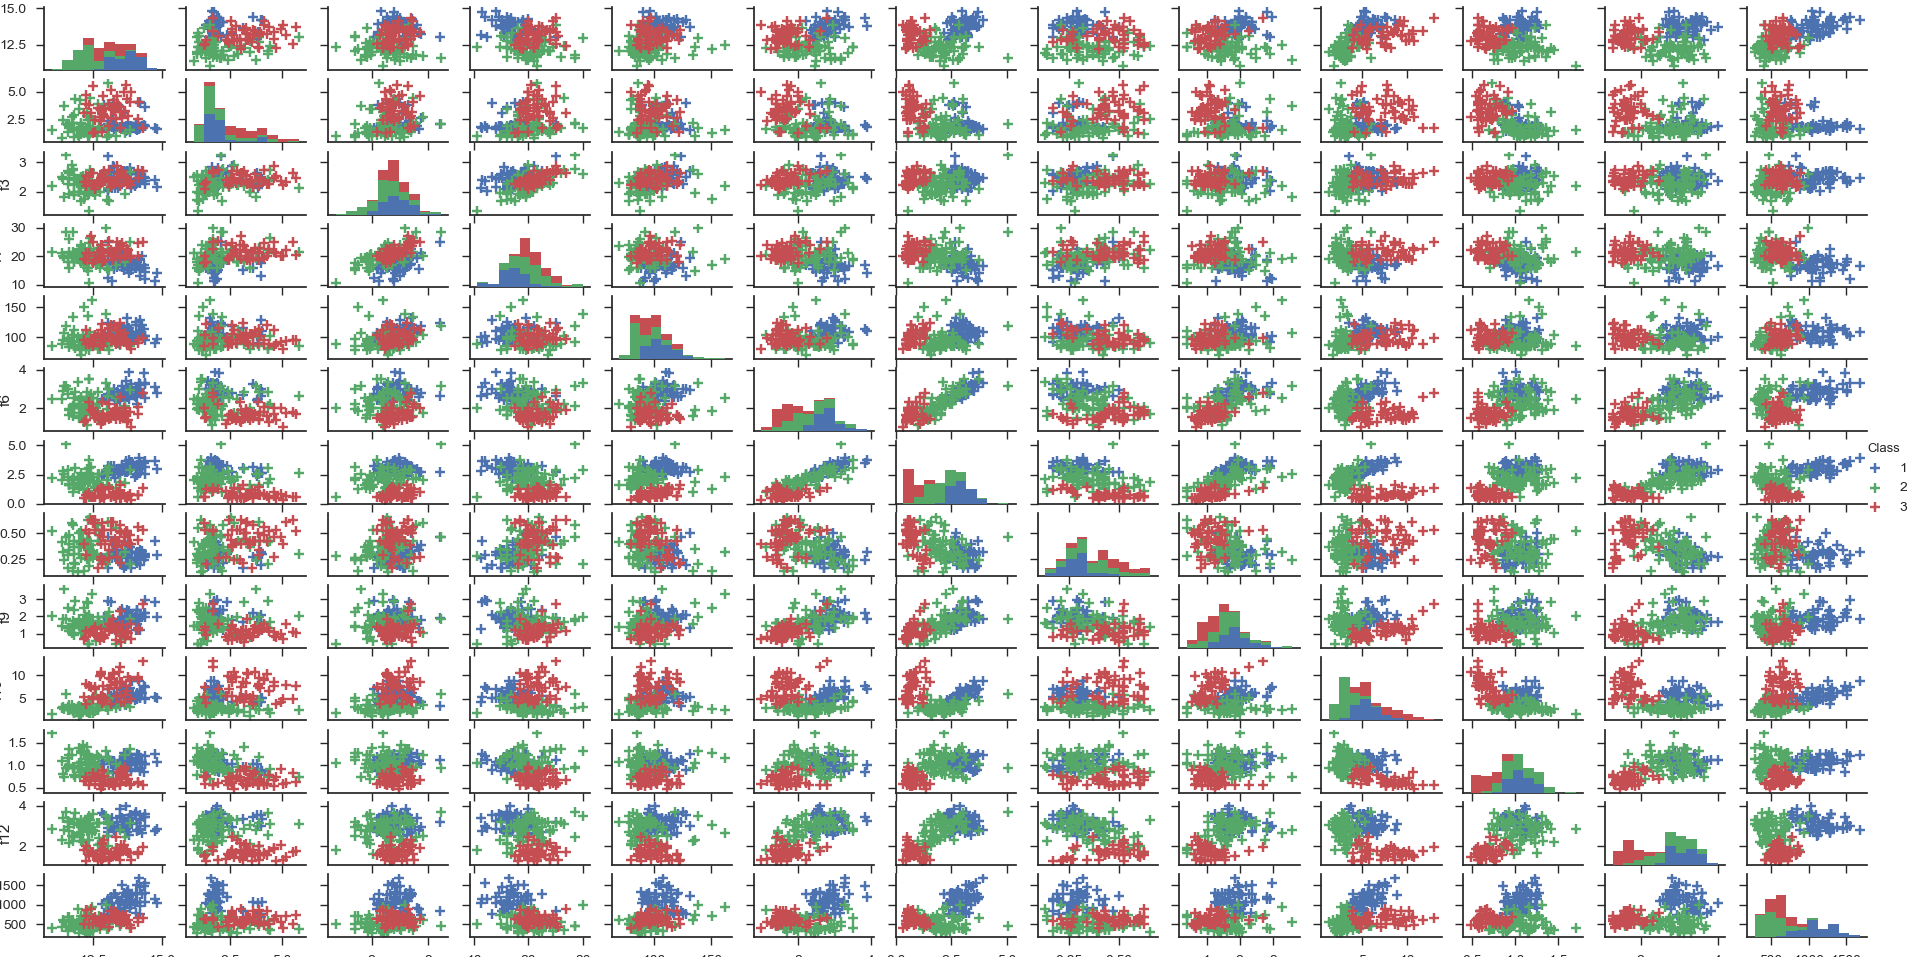
\includegraphics[width=1\textwidth]{dsWineCombined.png}
\caption{Rozkład cech dla zbioru Wine}
\end{figure}

\begin{figure}[H]
\centering
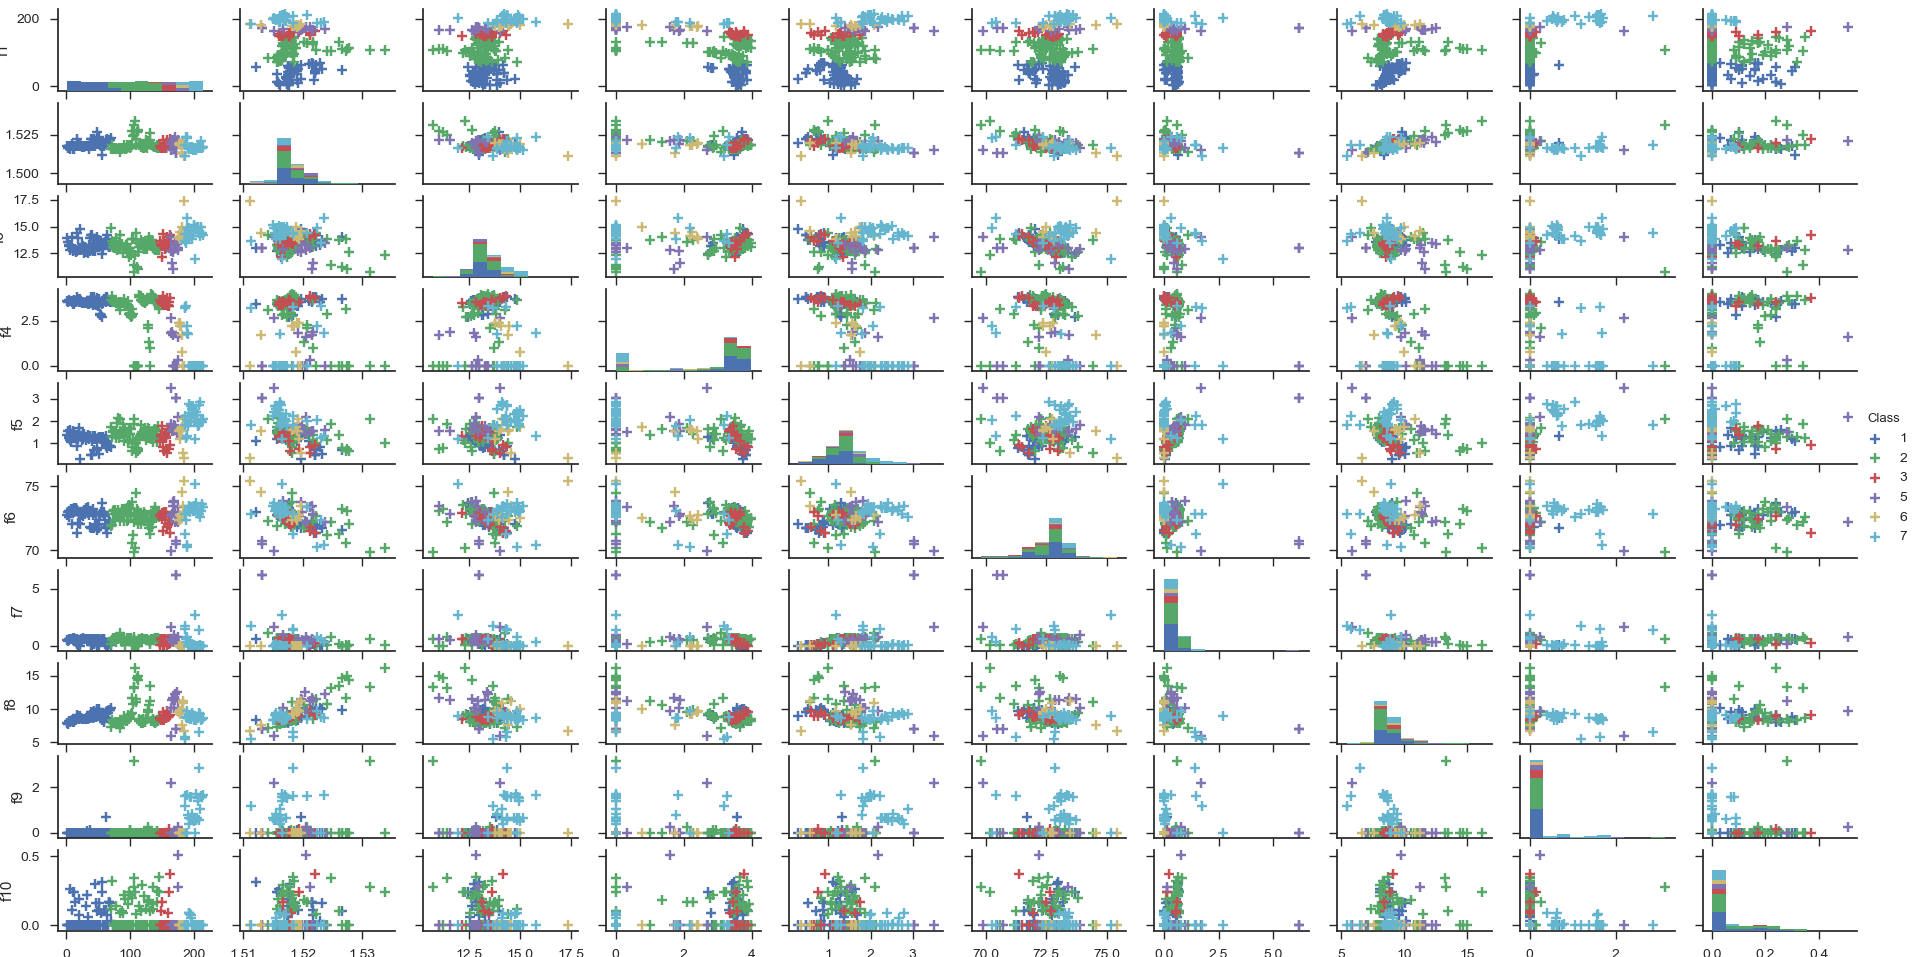
\includegraphics[width=1\textwidth]{dsGlassCombined.png}
\caption{Rozkład cech dla zbioru Glass}
\end{figure}

\begin{figure}[H]
\centering
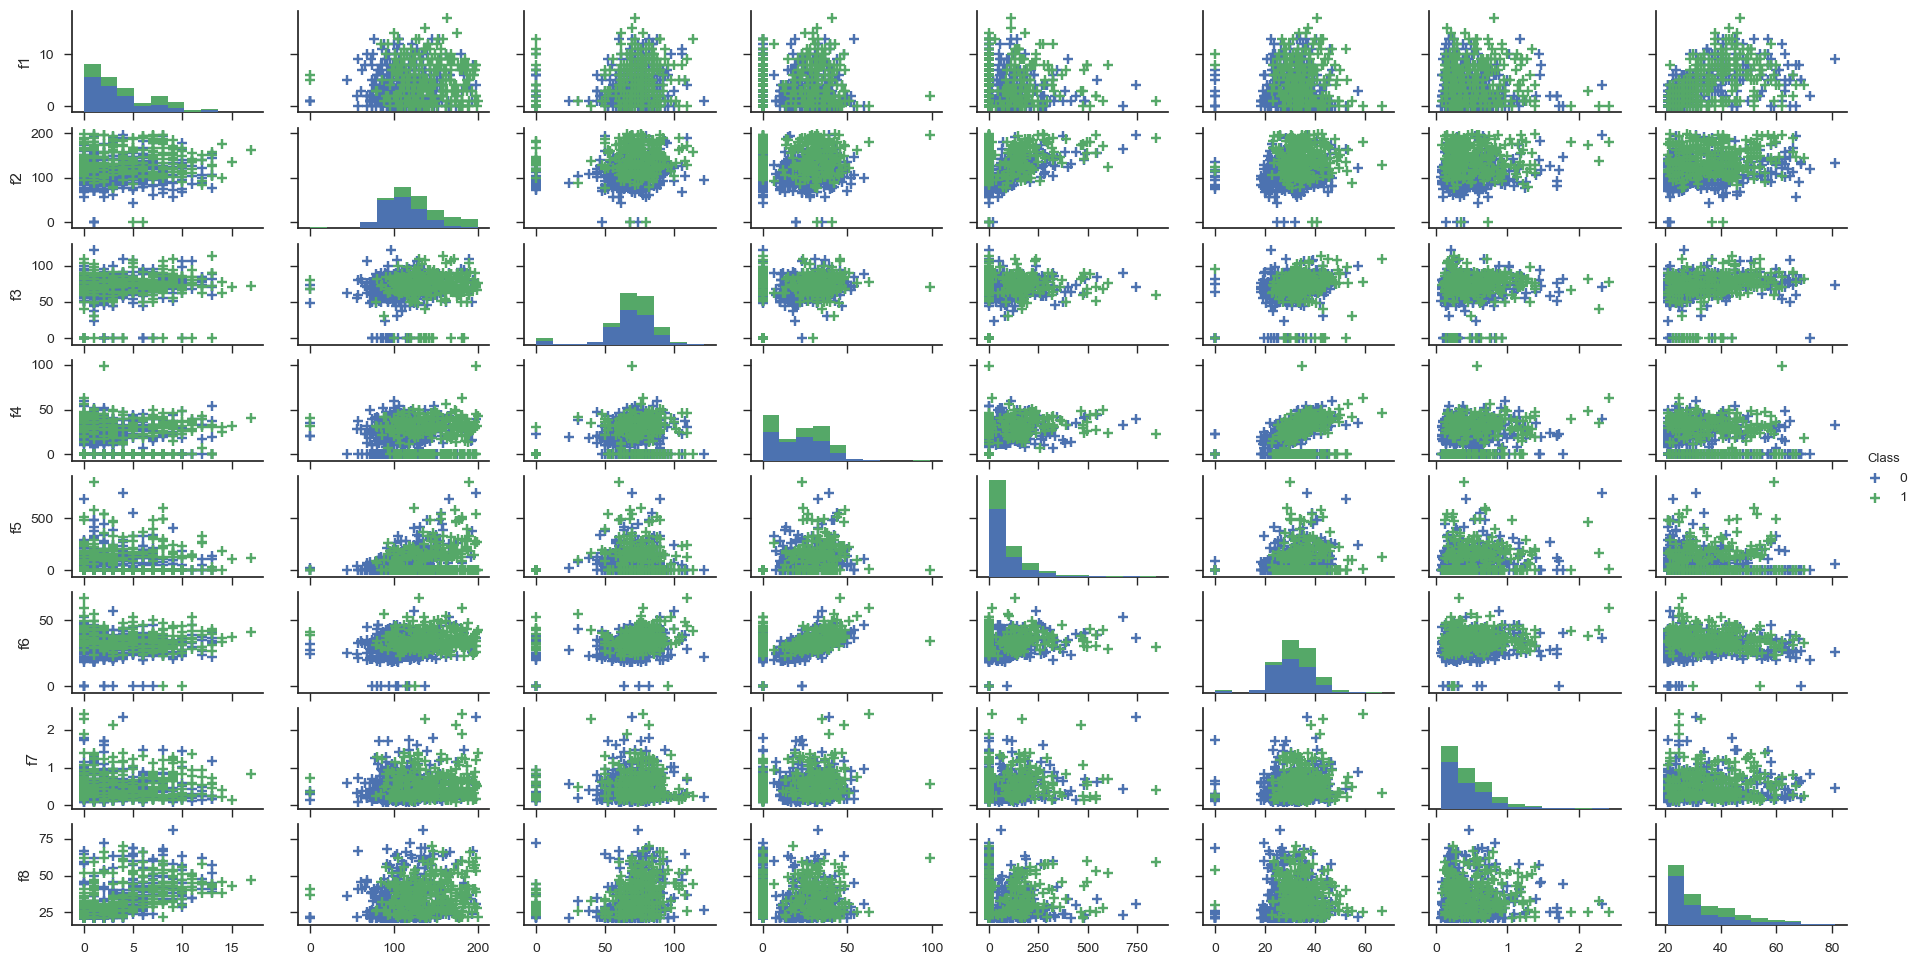
\includegraphics[width=1\textwidth]{dsDiabetesCombined.png}
\caption{Rozkład cech dla zbioru Diabetes}
\end{figure}




\section{Implementacja klasyfikatora i problem wygładzania}

Na podstawie zaprezentowanych wcześniej wzorów można stwierdzić, że w przypadku, gdy dana kombinacja cechy  i wartości nie wystąpi w zbiorze uczącym, wyzeruje ona prawdopodobieństwo klasyfikacji do danej klasy przy wystąpieniu cechy w czasie klasyfikacji właściwej. Z tym zjawiskiem można poradzić sobie poprzez wygładzenie danych, czyli eliminację zerowych prawdopodobieństw lub założenie, że dane mają rozkład normalny. W tym wypadku można skorzystać ze wzoru, który likwiduje zerowe prawdopodobieństwa.

$$ 
P(x_{i} \mid y) = 
\frac
{1}
{\sqrt{2 \pi \sigma^{2}_{y}}}
\exp
(- 
\frac
{(x_{i} - \mu_{y})^2)}
{2\sigma^{2}_{y}}
)
$$

Do badań wykorzystane zostaną dwie implementacje pochodzące z biblioteki \emph{sklearn}: \emph{GaussianNB} oraz \emph{MultinomialNB} ze współczynnikiem wygładzania  $\alpha$ = 1, który wykorzystuje \emph{wygładzanie laplace}.

\begin{python}
def getClassifireGausian(_df):
    featureVals = [x for x in _df if x != 'Class']
    gnb = GaussianNB()
    gnb.fit(_df[featureVals], _df['Class'])
    return gnb

def getClassifireMultinomial(_df):
    featureVals = [x for x in _df if x != 'Class']
    gnb = MultinomialNB(alpha=1.0)
    gnb.fit(_df[featureVals], _df['Class'])
    return gnb


def predict(_classifier, _df):
    featureVals = [x for x in _df if x != 'Class']
    y_pred = _classifier.predict(_df[featureVals])
    return y_pred
\end{python}

\section{Metody dyskretyzacji}
Jednym z celów zadania jest zbadanie wpływu dyskretyzacji danych na jakość klasyfikatora. W programie zaimplementowany zostały trzy rodzaje dyskretyzacji.
\begin{enumerate}
\item \emph{Equal width intervals}: podział zakresu wartości atrybutu ciągłego na k przedziałów o jednakowej szerokości.
\begin{python}
def equalWidth(_df):
    featureVals = [x for x in _df if x != 'Class']
    discretizedMap = {'Class': _df['Class']}

    for x in featureVals:
        discretizedMap[x] = pd.cut(_df[x], 5, labels=False)

    nFrame = pd.DataFrame.from_dict(discretizedMap)
    return nFrame
\end{python}
\item \emph{Equal frequency intervals }: podział zakresu wartości atrybutu ciągłego na k przedziałów, z których każdemu odpowiada możliwie tyle samo przykładów ze zbioru trenującego.
\begin{python}

def equalFreq(_df):
    featureVals = [x for x in _df if x != 'Class']
    discretizedMap = {'Class': _df['Class']}

    for x in featureVals:
        discretizedMap[x] = pd.qcut(_df[x], 5, labels=False, duplicates='drop')

    nFrame = pd.DataFrame.from_dict(discretizedMap)
    return nFrame
\end{python}

\item \emph{Minimum Description Length Binning}: bazująca na entropii metoda opracowana przez \emph{Usama Fayyad's}. Dokładny opis dostępny pod linkiem: 
\href{http://web.donga.ac.kr/kjunwoo/files/Multi%20interval%20discretization%20of%20continuous%20valued%20attributes%20for%20classification%20learning.pdf}{mdlp.}

\begin{python}
def discMdlp(_df):
    featureVals = [x for x in _df if x != 'Class']
    transformer = MDLP()
    discretizedMap = {'Class': _df['Class']}

    discret = transformer.fit_transform(_df[featureVals],_df['Class'])
    nFrame = pd.DataFrame(data=discret, columns=featureVals)
    nFrame.loc[:,'Class'] = pd.Series(_df['Class'])
    
    return nFrame
\end{python}
\end{enumerate}

Działanie poszczególnych metod dyskretyzacji dla instancji Glass przedstawiono poniżej.

\begin{figure}[H]
\centering

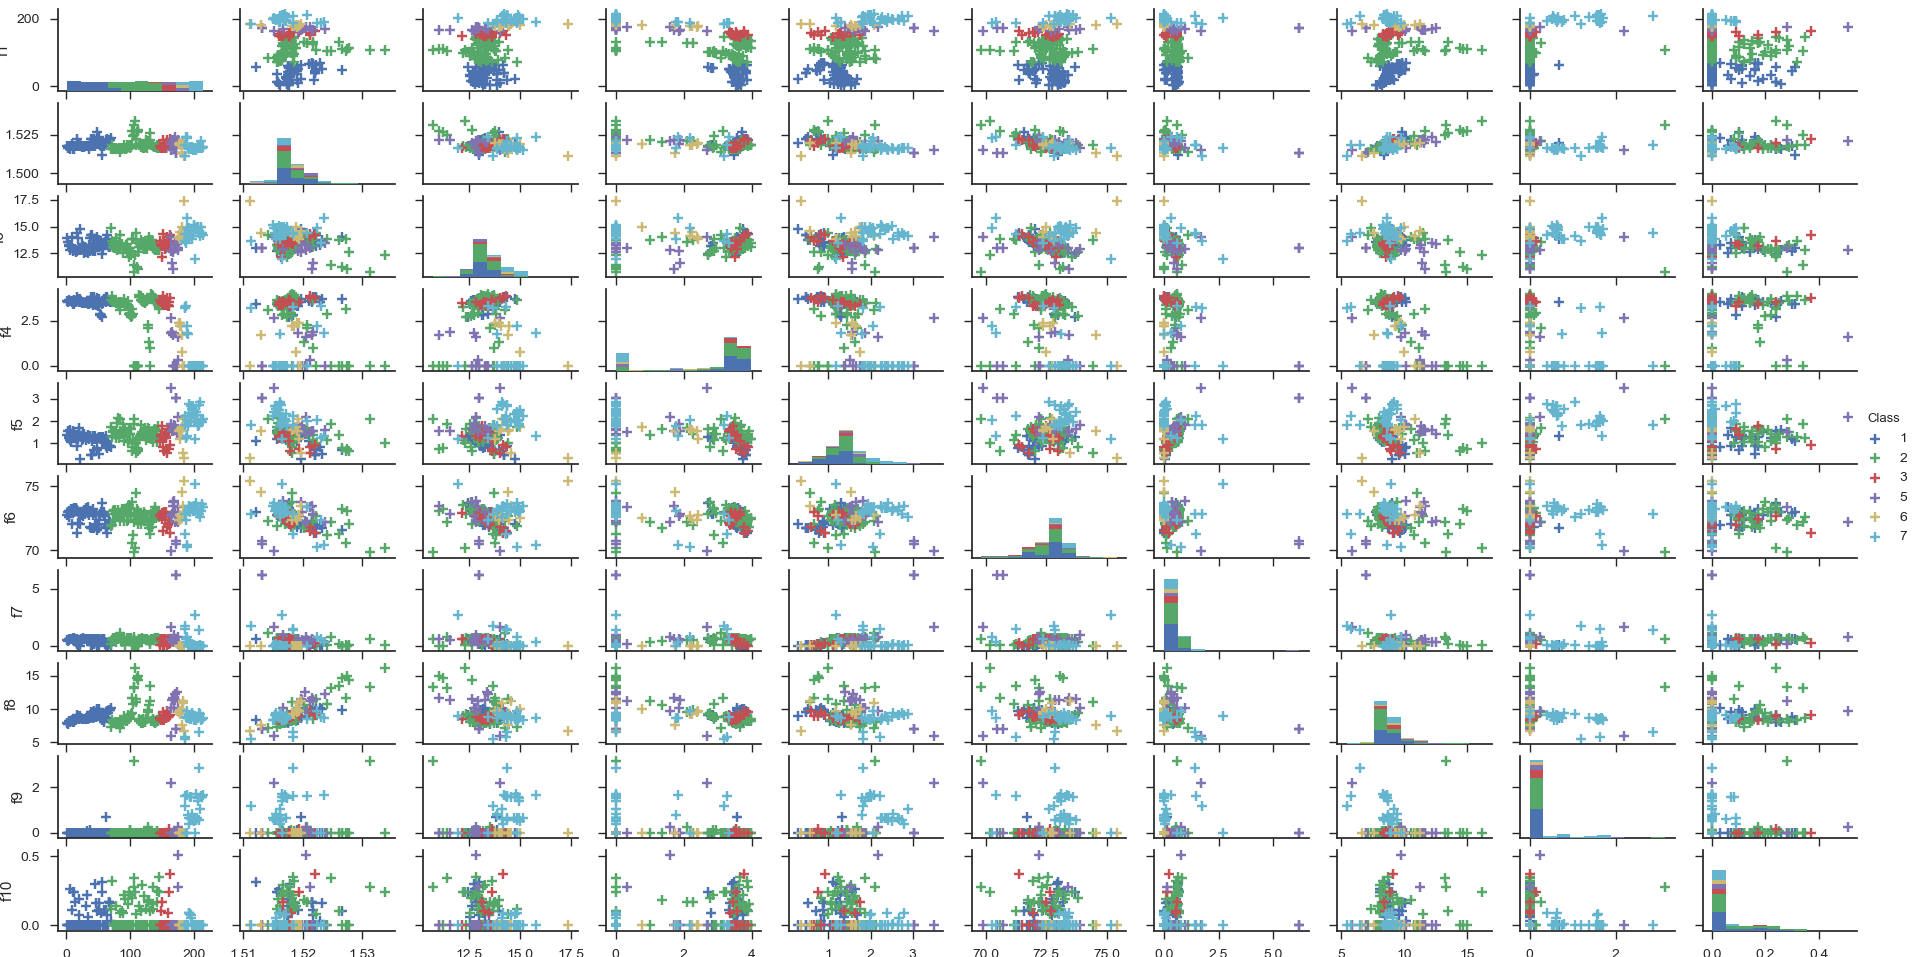
\includegraphics[width=1\textwidth]{dsGlassCombined.PNG}
\caption{Brak dyskretyzacji}
\end{figure}

\begin{figure}[H]
\centering
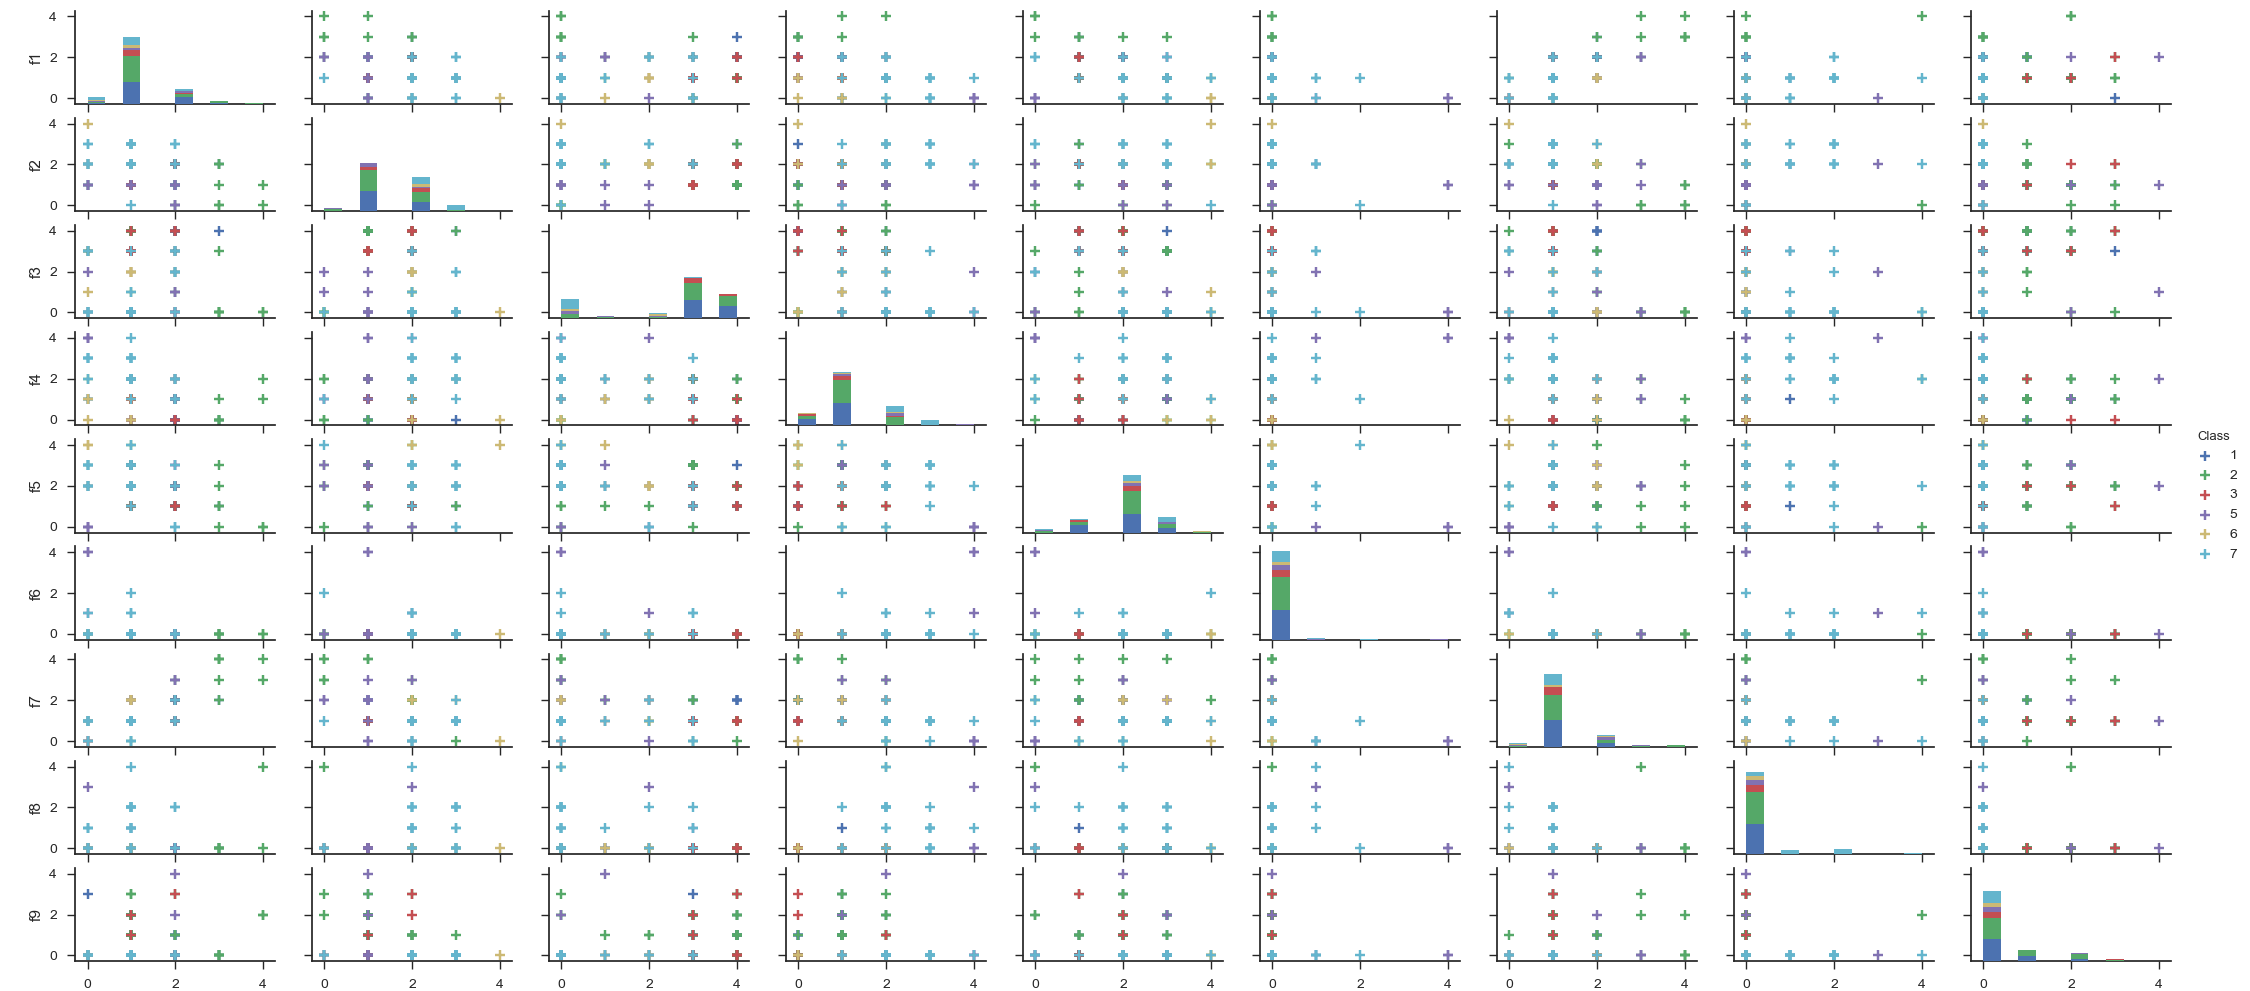
\includegraphics[width=1\textwidth]{dsGlassEqWidth.PNG}
\caption{Equal width}
\end{figure}


\begin{figure}[H]
\centering
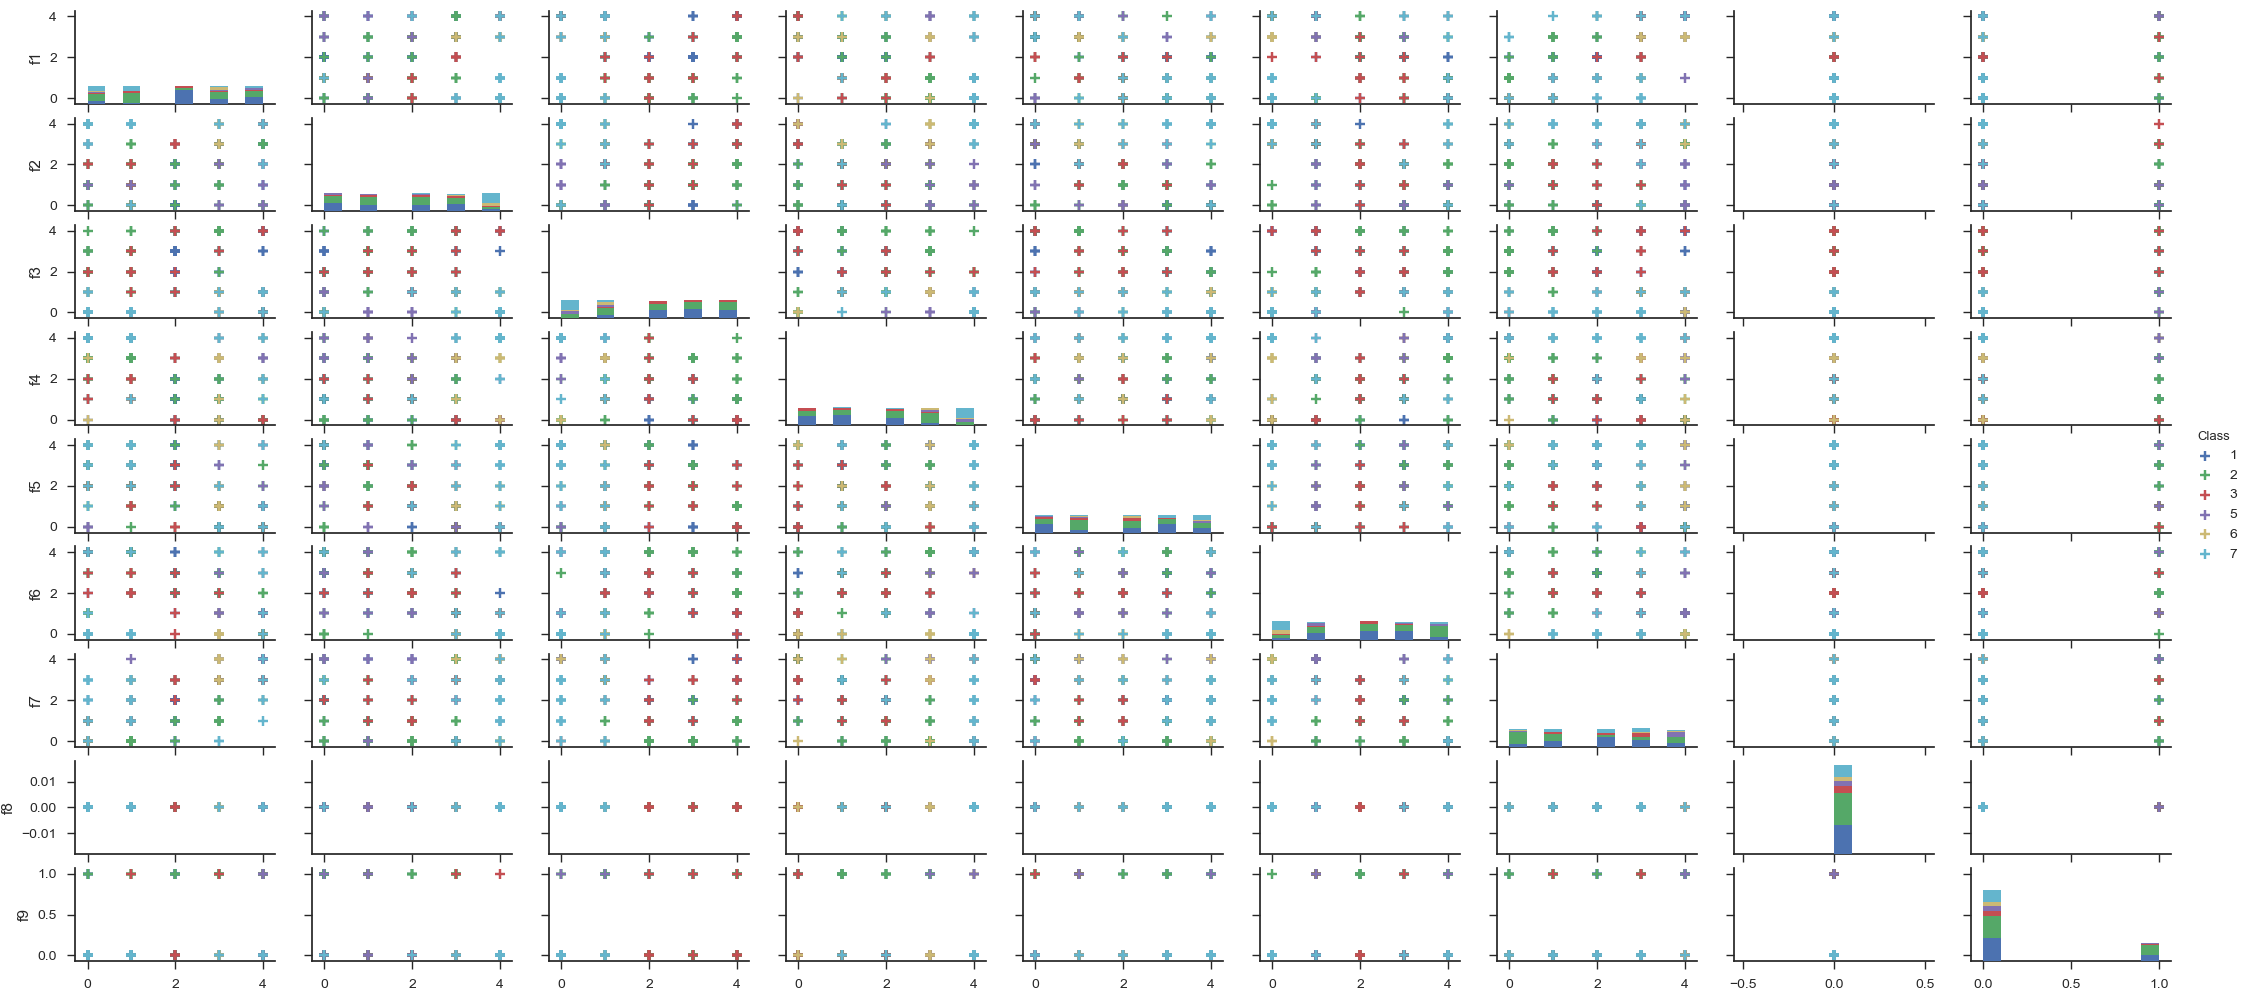
\includegraphics[width=1\textwidth]{dsGlassEqFreq.png}
\caption{Equal frequency}
\end{figure}

\begin{figure}[H]
\centering
\includegraphics[width=1\textwidth]{dsGlassMDLP.png}
\caption{MDLP}
\end{figure}

\section{Badanie metod kroswalidacji}
Do oceny klasyfikatora zostanie użyta metoda kroswalidacji z metodą podziału \emph{X-fold}. Polega ona na tym, że zbiór dzielimy na X w miarę możliwości równych części. W przypadku odmiany stratyfikowanej każda część zawiera możliwie tyle samo danych z każdej klasy. Jedna część zostanie użyta do oceny klasyfikatora, a pozostałe wejdą w skład zbioru trenującego. Następnie X razy zmianie ulegnie część do klasyfikacji, a cały proces zostanie powtórzony. 
Wpływ rodzaju kroswalidacji dla różnych zbiorów przedstawiono w poniższych tabelach. 

\begin{tabular}{ |p{2.3cm}||p{2.5cm}|p{2.5cm}|p{2.5cm}|p{2.5cm}| }
 \hline
 Ilość części & Aaccracy & Precision & Recall & fscore\\
 \hline
\hline
\multicolumn{5}{|c|}{Instancja Wine}\\
\hline
\hline
\multicolumn{5}{|c|}{Brak randomizacji, brak stratyfikacji}\\
\hline
2&0.37& 0.15& 0.37& 0.21\\
3&0.30& 0.13& 0.30& 0.18\\
4&0.66& 0.66& 0.66& 0.60\\
5&0.93& 0.93& 0.93& 0.93\\
6&0.93& 0.93& 0.93& 0.93\\
7&0.93& 0.93& 0.93& 0.93\\
8&0.96& 0.96& 0.96& 0.96\\
9&0.95& 0.95& 0.95& 0.95\\
10&0.96& 0.96& 0.96& 0.96\\
\hline
\multicolumn{5}{|c|}{Randomizacja, brak stratyfikacji}\\
\hline
2&0.98& 0.98& 0.98& 0.98\\
3&0.98& 0.98& 0.98& 0.98\\
4&0.97& 0.97& 0.97& 0.97\\
5&0.97& 0.97& 0.97& 0.97\\
6&0.98& 0.98& 0.98& 0.98\\
7&0.97& 0.97& 0.97& 0.97\\
8&0.97& 0.97& 0.97& 0.97\\
9&0.96& 0.96& 0.96& 0.96\\
10&0.98& 0.98& 0.98& 0.98\\
\hline
\multicolumn{5}{|c|}{Brak randomizacji, stratyfikacja}\\
\hline
2&0.97& 0.97& 0.97& 0.97\\
3&0.96& 0.96& 0.96& 0.96\\
4&0.96& 0.96& 0.96& 0.96\\
5&0.95& 0.95& 0.95& 0.95\\
6&0.96& 0.96& 0.96& 0.96\\
7&0.96& 0.96& 0.96& 0.96\\
8&0.96& 0.96& 0.96& 0.96\\
9&0.95& 0.95& 0.95& 0.95\\
10&0.96& 0.96& 0.96& 0.96\\
\hline
\multicolumn{5}{|c|}{Randomizacja, stratyfikacja}\\
\hline
2&0.97& 0.97& 0.97& 0.97\\
3&0.96& 0.96& 0.96& 0.96\\
4&0.96& 0.96& 0.96& 0.96\\
5&0.95& 0.95& 0.95& 0.95\\
6&0.96& 0.96& 0.96& 0.96\\
7&0.96& 0.96& 0.96& 0.96\\
8&0.96& 0.96& 0.96& 0.96\\
9&0.95& 0.95& 0.95& 0.95\\
10&0.96& 0.96& 0.96& 0.96\\
\hline
\end{tabular}

\begin{tabular}{ |p{2.3cm}||p{2.5cm}|p{2.5cm}|p{2.5cm}|p{2.5cm}| }
\hline
\multicolumn{5}{|c|}{Instancja Glass}\\
\hline
\hline
\multicolumn{5}{|c|}{Brak randomizacji, brak stratyfikacji}\\
\hline
2&0.09& 0.08& 0.09& 0.08\\
3&0.23& 0.16& 0.23& 0.19\\
4&0.13& 0.12& 0.13& 0.13\\
5&0.20& 0.25& 0.20& 0.21\\
6&0.12& 0.18 & 0.12& 0.13\\
7&0.28& 0.33& 0.28& 0.28\\
8&0.17& 0.20& 0.17& 0.17\\
9&0.25& 0.37& 0.25& 0.28\\
10&0.33& 0.41& 0.33& 0.34\\
\hline
\multicolumn{5}{|c|}{Randomizacja, brak stratyfikacji}\\
\hline
2&0.40& 0.48& 0.40& 0.40\\
3&0.43& 0.53& 0.43& 0.46\\
4&0.40& 0.48& 0.40& 0.40\\
5&0.40& 0.45& 0.40& 0.40\\
6&0.46& 0.48& 0.46& 0.44\\
7&0.43& 0.45& 0.43& 0.41\\
8&0.43& 0.49& 0.43& 0.42\\
9&0.44& 0.48& 0.44& 0.43\\
10&0.45& 0.46& 0.45& 0.42\\
\hline
\multicolumn{5}{|c|}{Brak randomizacji, stratyfikacja}\\
\hline
2&0.36& 0.47& 0.36& 0.39\\
3&0.37& 0.44& 0.37& 0.38\\
4&0.39& 0.47& 0.39& 0.40\\
5&0.33& 0.38& 0.33& 0.34\\
6&0.41& 0.44& 0.41& 0.40\\
7&0.39& 0.39& 0.39& 0.37\\
8&0.42& 0.42& 0.42& 0.39\\
9&0.44& 0.44& 0.44& 0.42\\
10&0.43& 0.43& 0.43& 0.41\\
\hline
\multicolumn{5}{|c|}{Randomizacja, stratyfikacja}\\
\hline
2&0.36& 0.47& 0.36& 0.39\\
3&0.37& 0.44& 0.37& 0.38\\
4&0.39& 0.47& 0.39& 0.40\\
5&0.33& 0.38& 0.33& 0.34\\
6&0.41& 0.44& 0.41& 0.40\\
7&0.39& 0.39& 0.39& 0.37\\
8&0.42& 0.42& 0.42& 0.39\\
9&0.44& 0.44& 0.44& 0.42\\
10&0.43& 0.43& 0.43& 0.41\\
\hline
\end{tabular}

\begin{tabular}{ |p{2.3cm}||p{2.5cm}|p{2.5cm}|p{2.5cm}|p{2.5cm}| }
\hline
\multicolumn{5}{|c|}{Instancja Diabetes}\\
\hline
\hline
\multicolumn{5}{|c|}{Brak randomizacji, brak stratyfikacji}\\
\hline
2&0.75& 0.66& 0.60& 0.63\\
3&0.74& 0.64& 0.58& 0.61\\
4&0.75& 0.66& 0.60& 0.63\\
5&0.75& 0.66& 0.59& 0.62\\
6&0.75& 0.66& 0.60& 0.63\\
7&0.75& 0.66& 0.59& 0.62\\
8&0.75& 0.66& 0.59& 0.62\\
9&0.75& 0.66& 0.60& 0.63\\
10&0.75& 0.66& 0.59& 0.62\\
\hline
\multicolumn{5}{|c|}{Randomizacja, brak stratyfikacji}\\
\hline
2&0.75& 0.65& 0.59& 0.62\\
3&0.75& 0.65& 0.60& 0.62\\
4&0.75& 0.65& 0.60& 0.63\\
5&0.76& 0.67& 0.60& 0.63\\
6&0.75& 0.66& 0.60& 0.63\\
7&0.75& 0.66& 0.59& 0.62\\
8&0.74& 0.65& 0.59& 0.62\\
9&0.75& 0.66& 0.60& 0.63\\
10&0.75& 0.65& 0.59& 0.62\\
\hline
\multicolumn{5}{|c|}{Brak randomizacji, stratyfikacja}\\
\hline
2&0.75& 0.66& 0.60& 0.63\\
3&0.74& 0.64& 0.58& 0.61\\
4&0.75& 0.65& 0.59& 0.62\\
5&0.75& 0.66& 0.58& 0.62\\
6&0.75& 0.65& 0.60& 0.63\\
7&0.75& 0.66& 0.59& 0.62\\
8&0.75& 0.66& 0.59& 0.62\\
9&0.75& 0.65& 0.59& 0.62\\
10&0.75& 0.67& 0.59& 0.62\\
\hline
\multicolumn{5}{|c|}{Randomizacja, stratyfikacja}\\
\hline
2&0.75& 0.66& 0.60& 0.63\\
3&0.74& 0.64& 0.58& 0.61\\
4&0.75& 0.65& 0.59& 0.62\\
5&0.75& 0.66& 0.58& 0.62\\
6&0.75& 0.65& 0.60& 0.63\\
7&0.75& 0.66& 0.59& 0.62\\
8&0.75& 0.66& 0.59& 0.62\\
9&0.75& 0.65& 0.59& 0.62\\
10&0.75& 0.67& 0.59& 0.62\\
 \hline
\end{tabular}
\vspace{5mm}

W przypadku próby kroswalidacji stratyfikowanej dla instancji, w której któryś z atrybutów występuje mniej razy niż ilość części, na które chcemy dokonać podziału, otrzymamy następujące ostrzeżenie:
\textbf{The least populated class in y has only 9 members, which is too few.The minimum number of members in any class cannot be less than n\_splits}, a w jednym ze zbiorów egzaminacyjnych obiekt z jednej klasy nie wystąpi.
Widać wyraźnie, że w przypadku kroswalidacji stratyfikowanej zmiana ilości części nie wpływa na wyniki klasyfikacji znacząco. W przypadku braku stratyfikacji nie ma sensu oceniać klasyfikatora bez randomizacji, ponieważ wszystko wtedy zależy od kolejności danych. Najlepszą metodą oceny jest kroswalidacja startyfikowana z randomizacją i to właśnie ta metoda będzie używana do oceny klasyfikatorów. 



\section{Porównanie działania algorytmów}
Dla wszystkich ze zbiorów zbadano jakość klasyfikatorów w zależności od sposobu liczenia prawdopodobieństwa, a w przypadku użycia \emph{multinomialNB}, wpływ różnych metod dyskretyzacji na zmianę jakości klasyfikatora. Badania wykonano dla wszystkich zbiorów. W przypadku dyskretyzacji dla każdego ze zbiorów próbowano dobrać optymalne parametry algorytmów, a poniżej przedstawiono najlepsze rezultaty.

\begin{figure}[H]
\centering
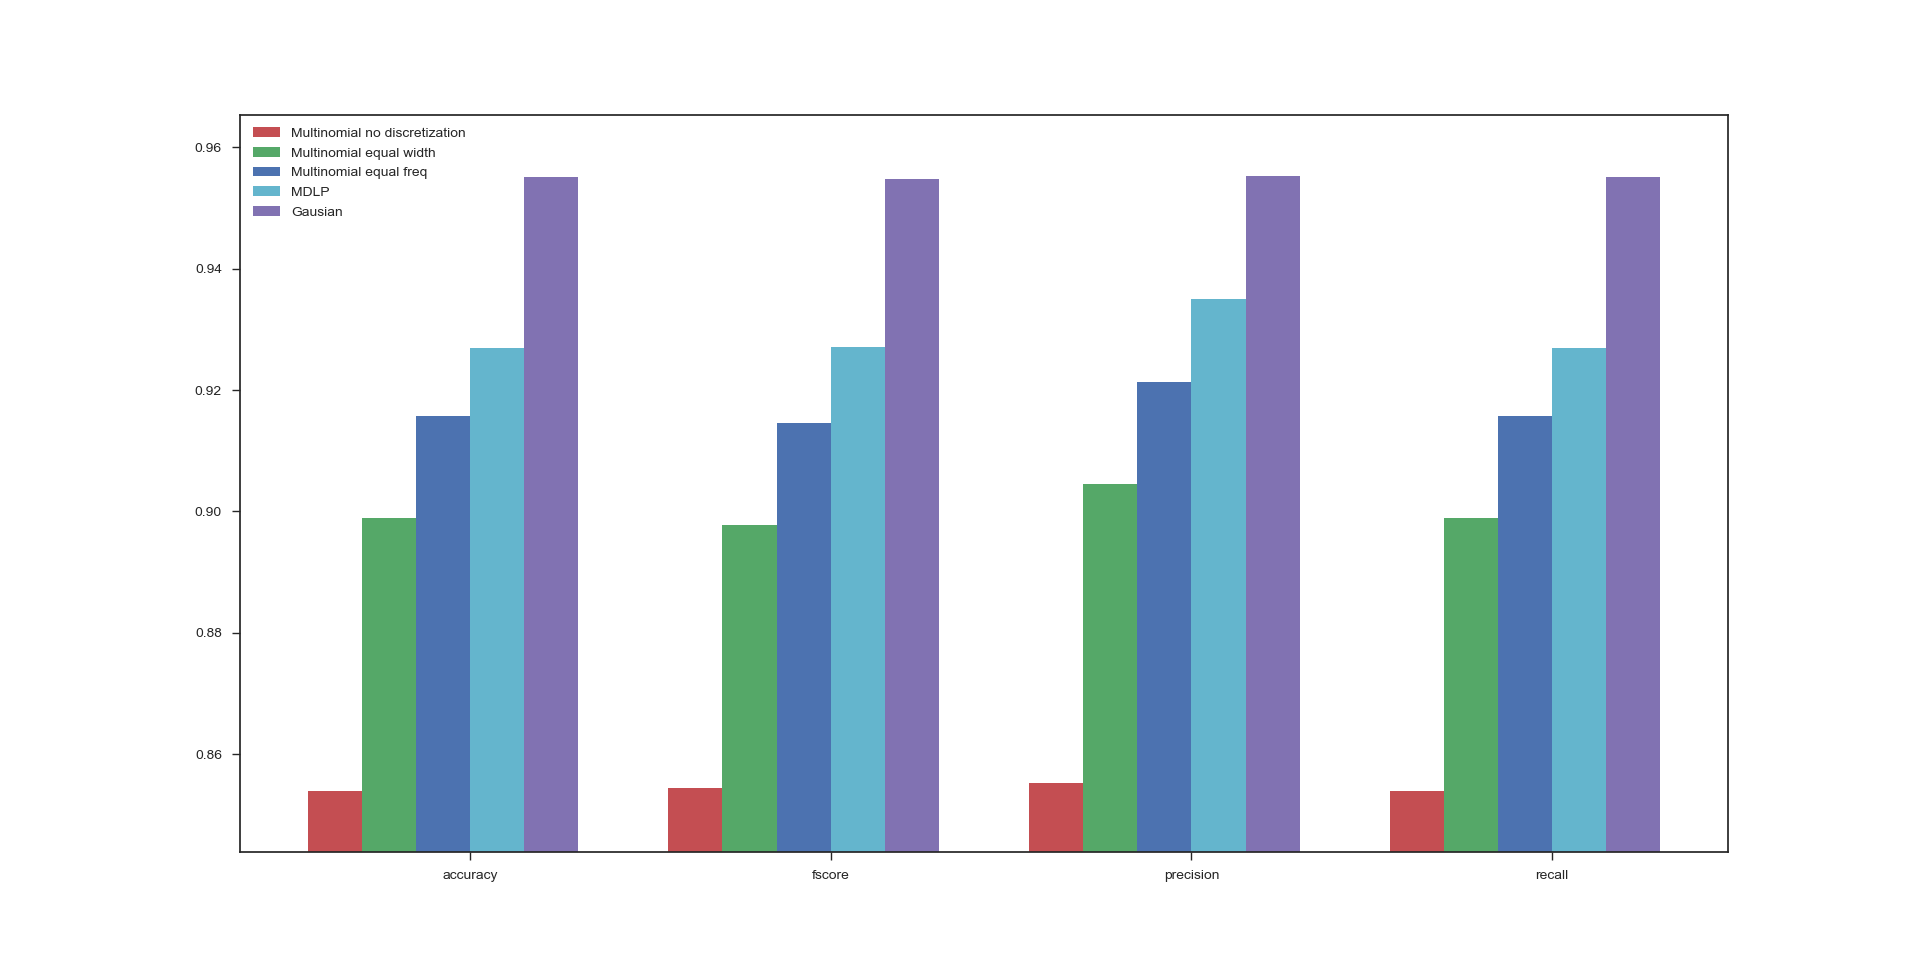
\includegraphics[width=1\textwidth]{wineStats.png}
\caption{Statystyki dla instancji Wine}
\end{figure}

\begin{figure}[H]
\centering
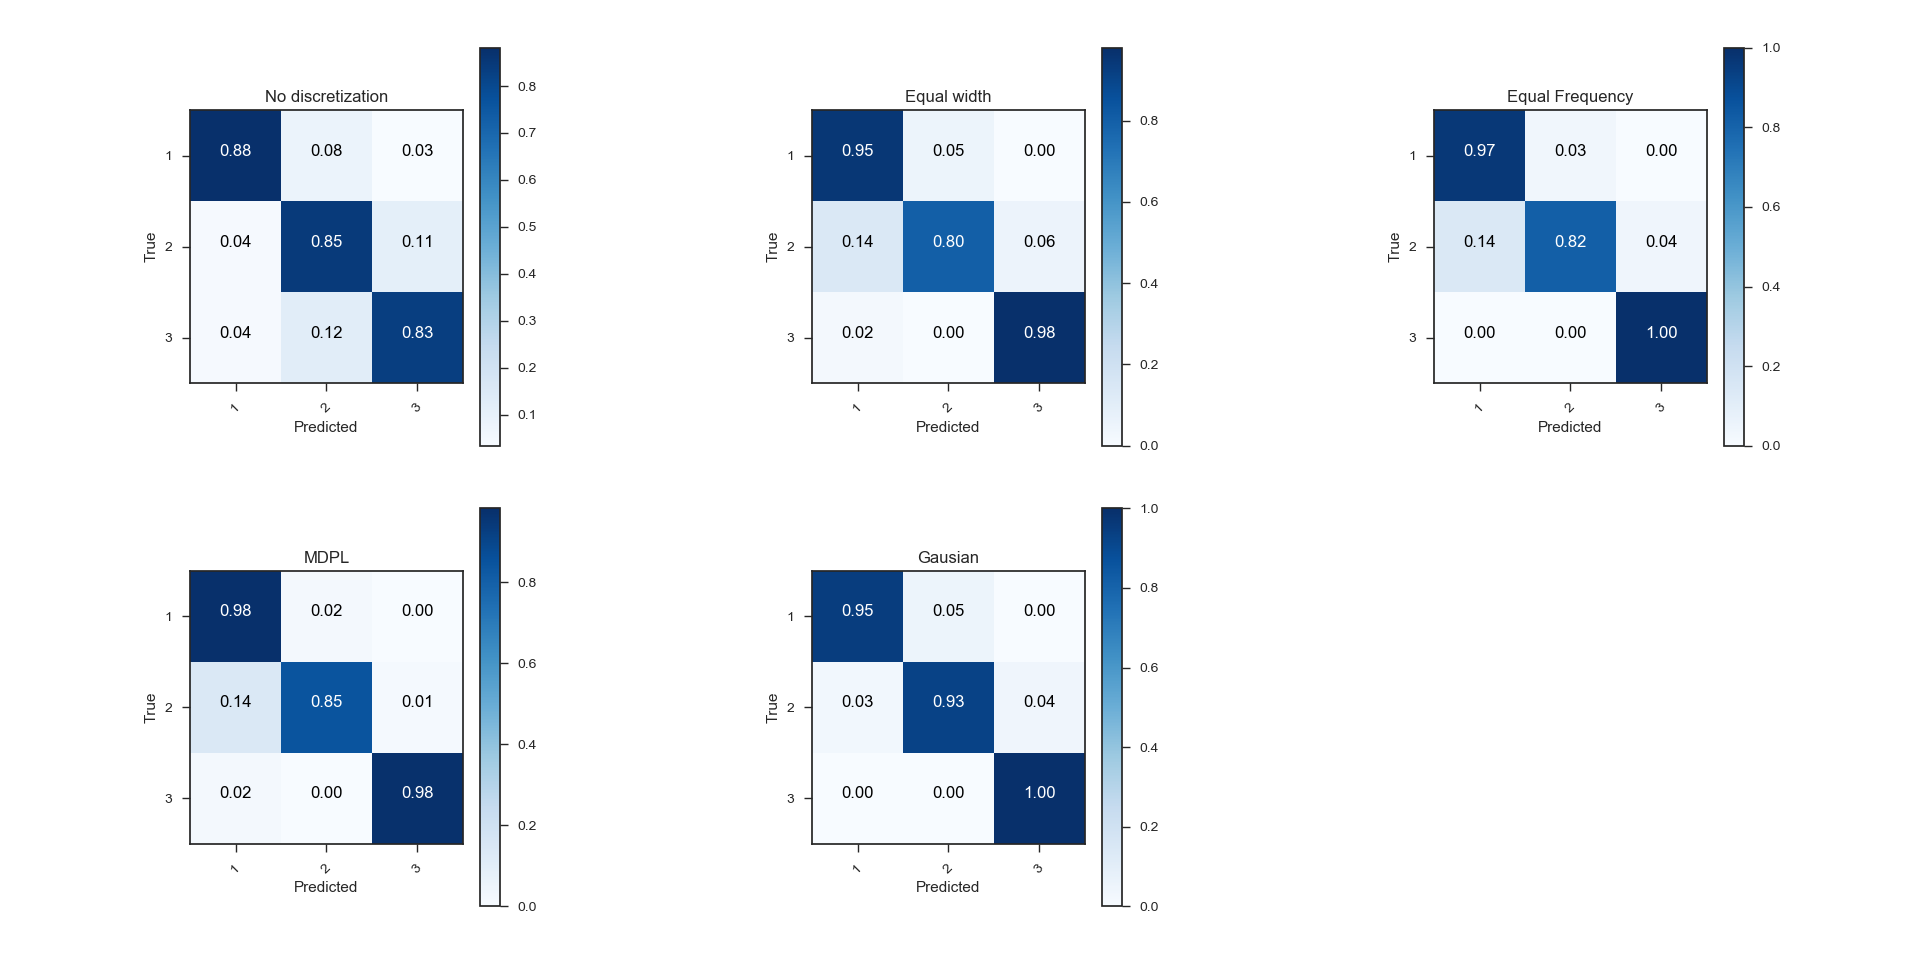
\includegraphics[width=1\textwidth]{wineCM.png}
\caption{Confusion Matrix dla instancji Wine}
\end{figure}

\begin{figure}[H]
\centering
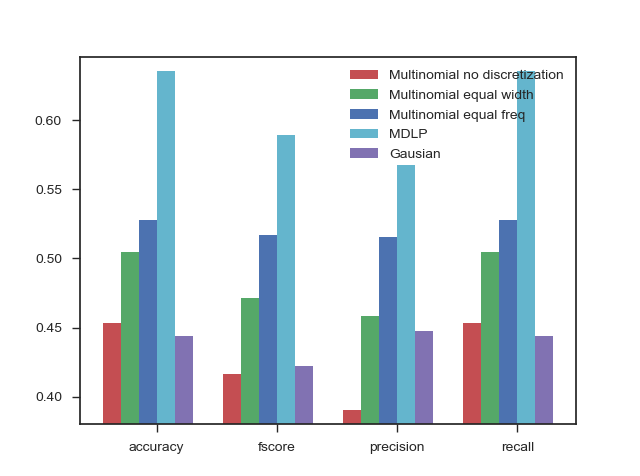
\includegraphics[width=1\textwidth]{glassStats.png}
\caption{Statystyki dla instancji Glass}
\end{figure}

\begin{figure}[H]
\centering
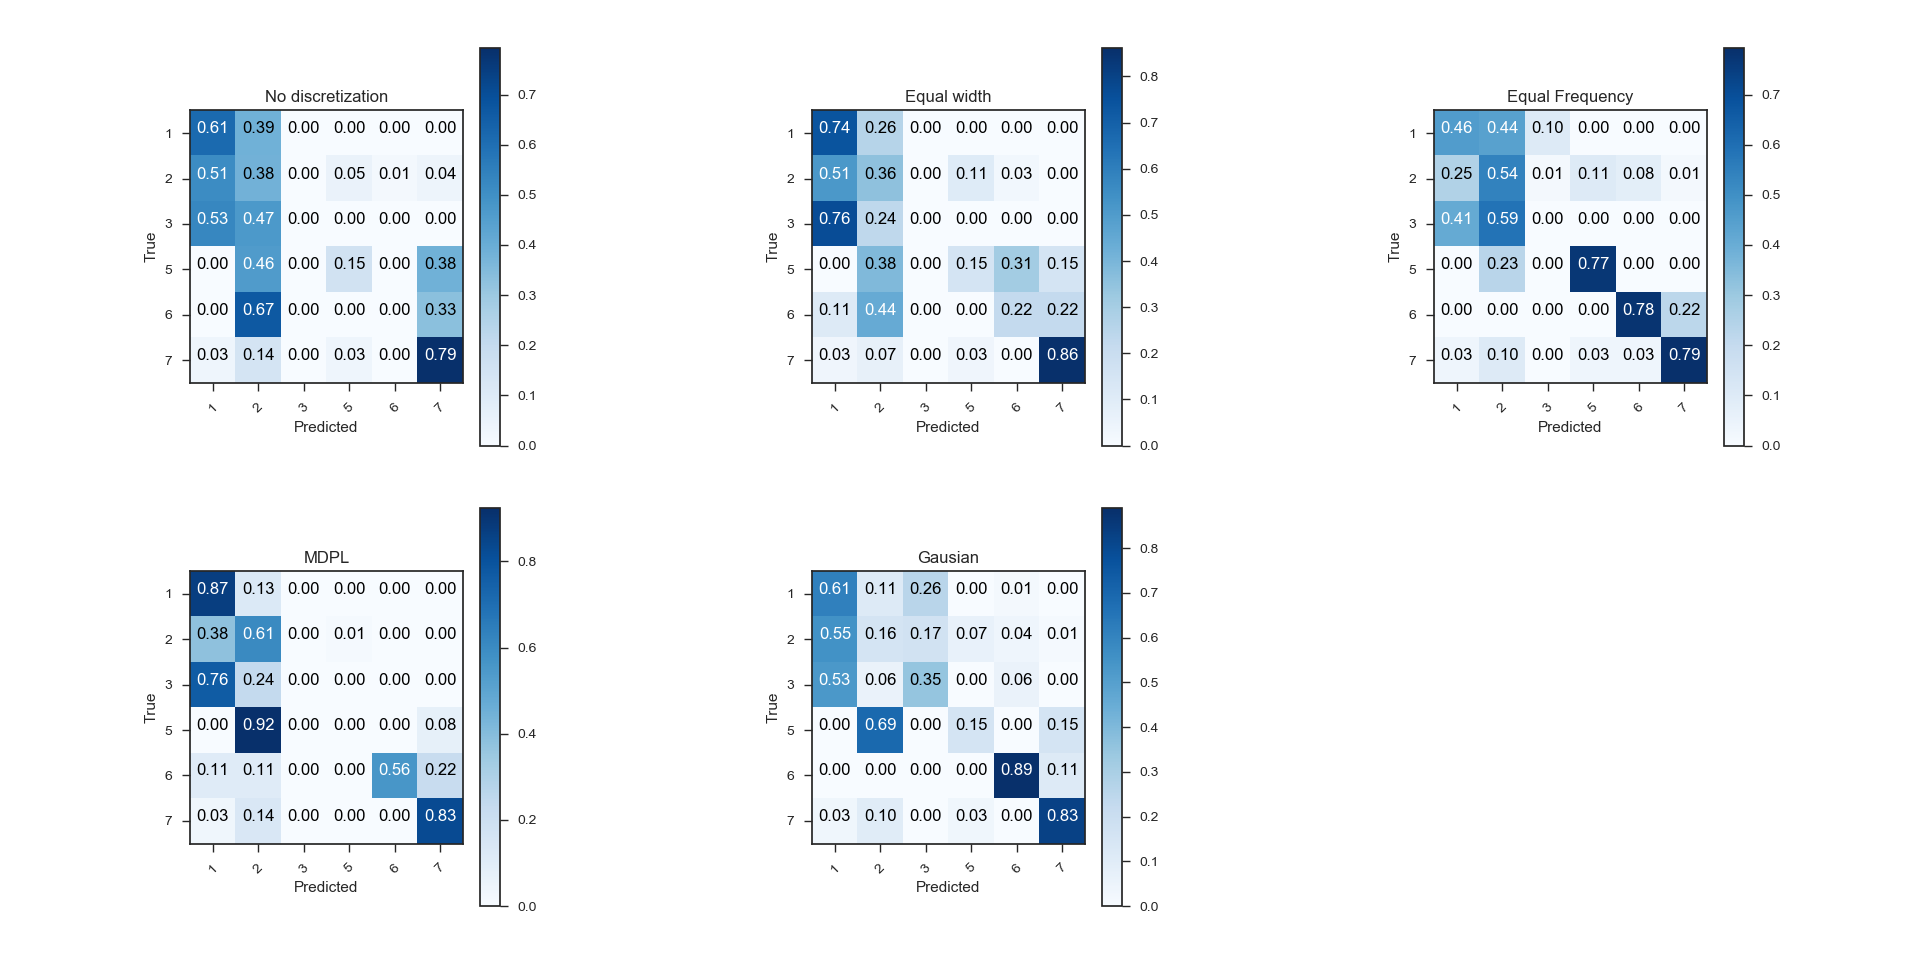
\includegraphics[width=1\textwidth]{glassCM.png}
\caption{Confusion Matrix dla instancji Glass}
\end{figure}

\begin{figure}[H]
\centering
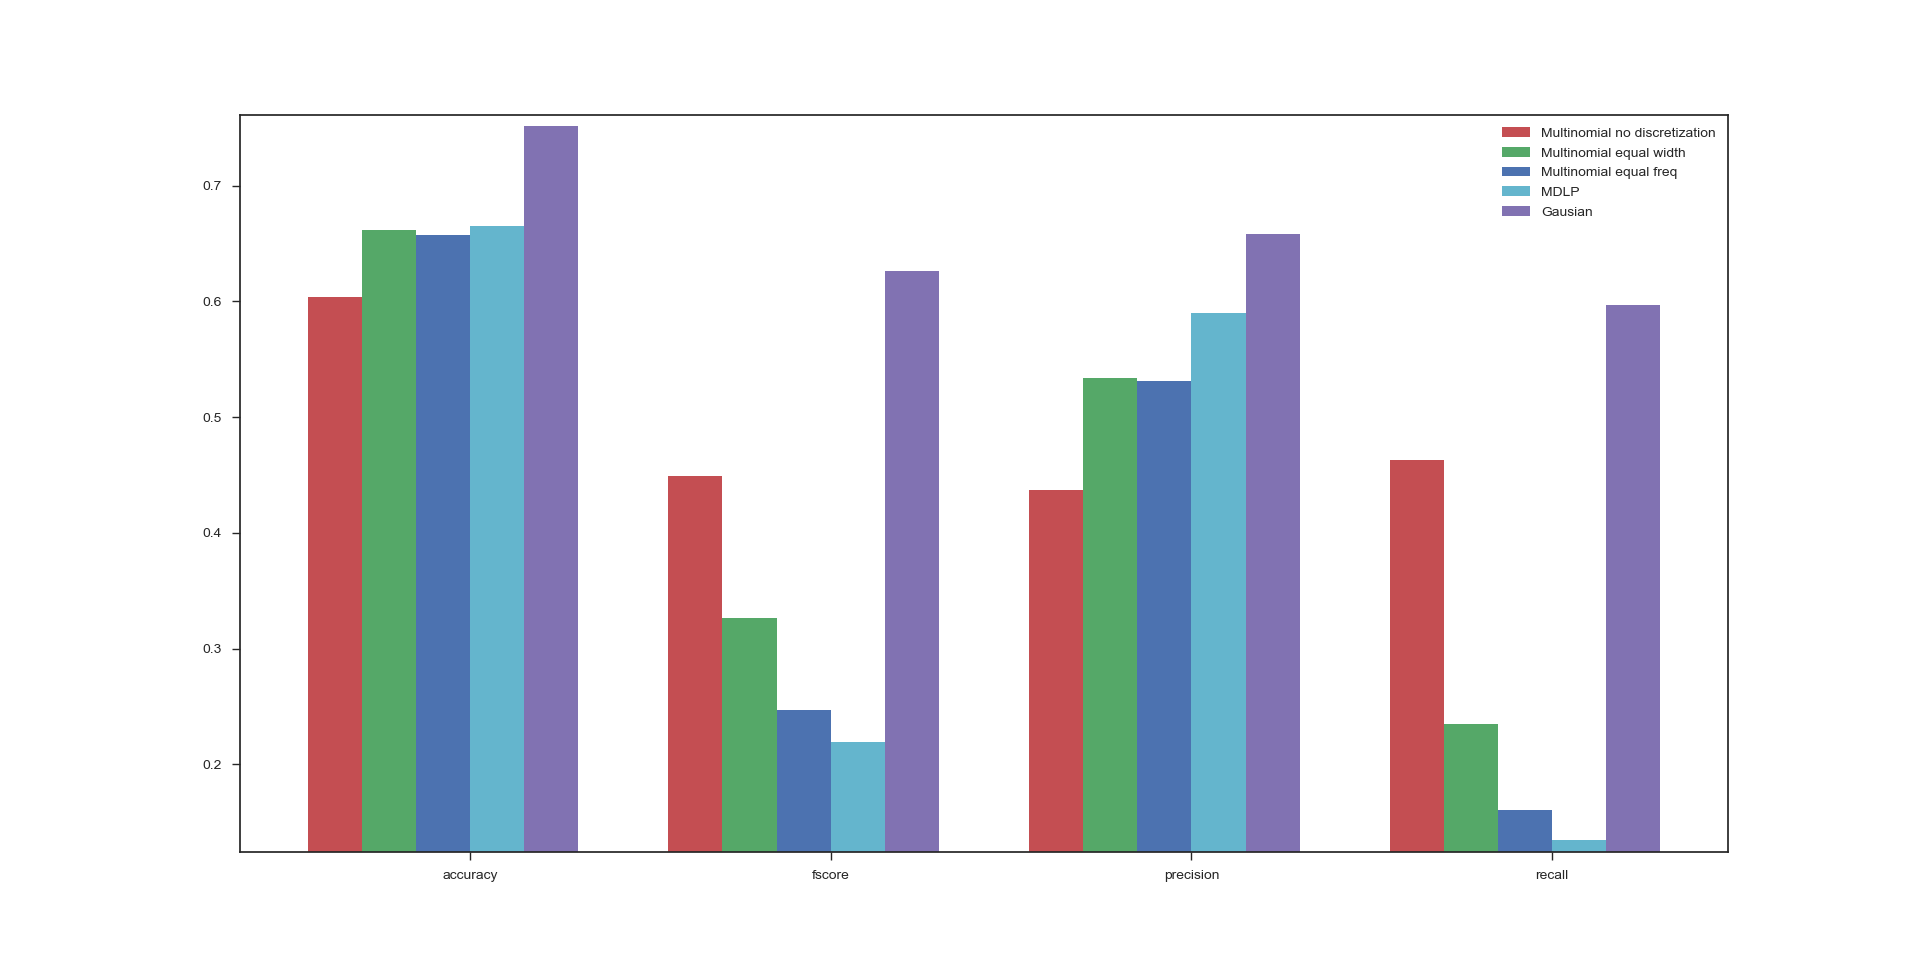
\includegraphics[width=1\textwidth]{diabetesStats.png}
\caption{Statystyki dla instancji Diabetes}
\end{figure}

\begin{figure}[H]
\centering
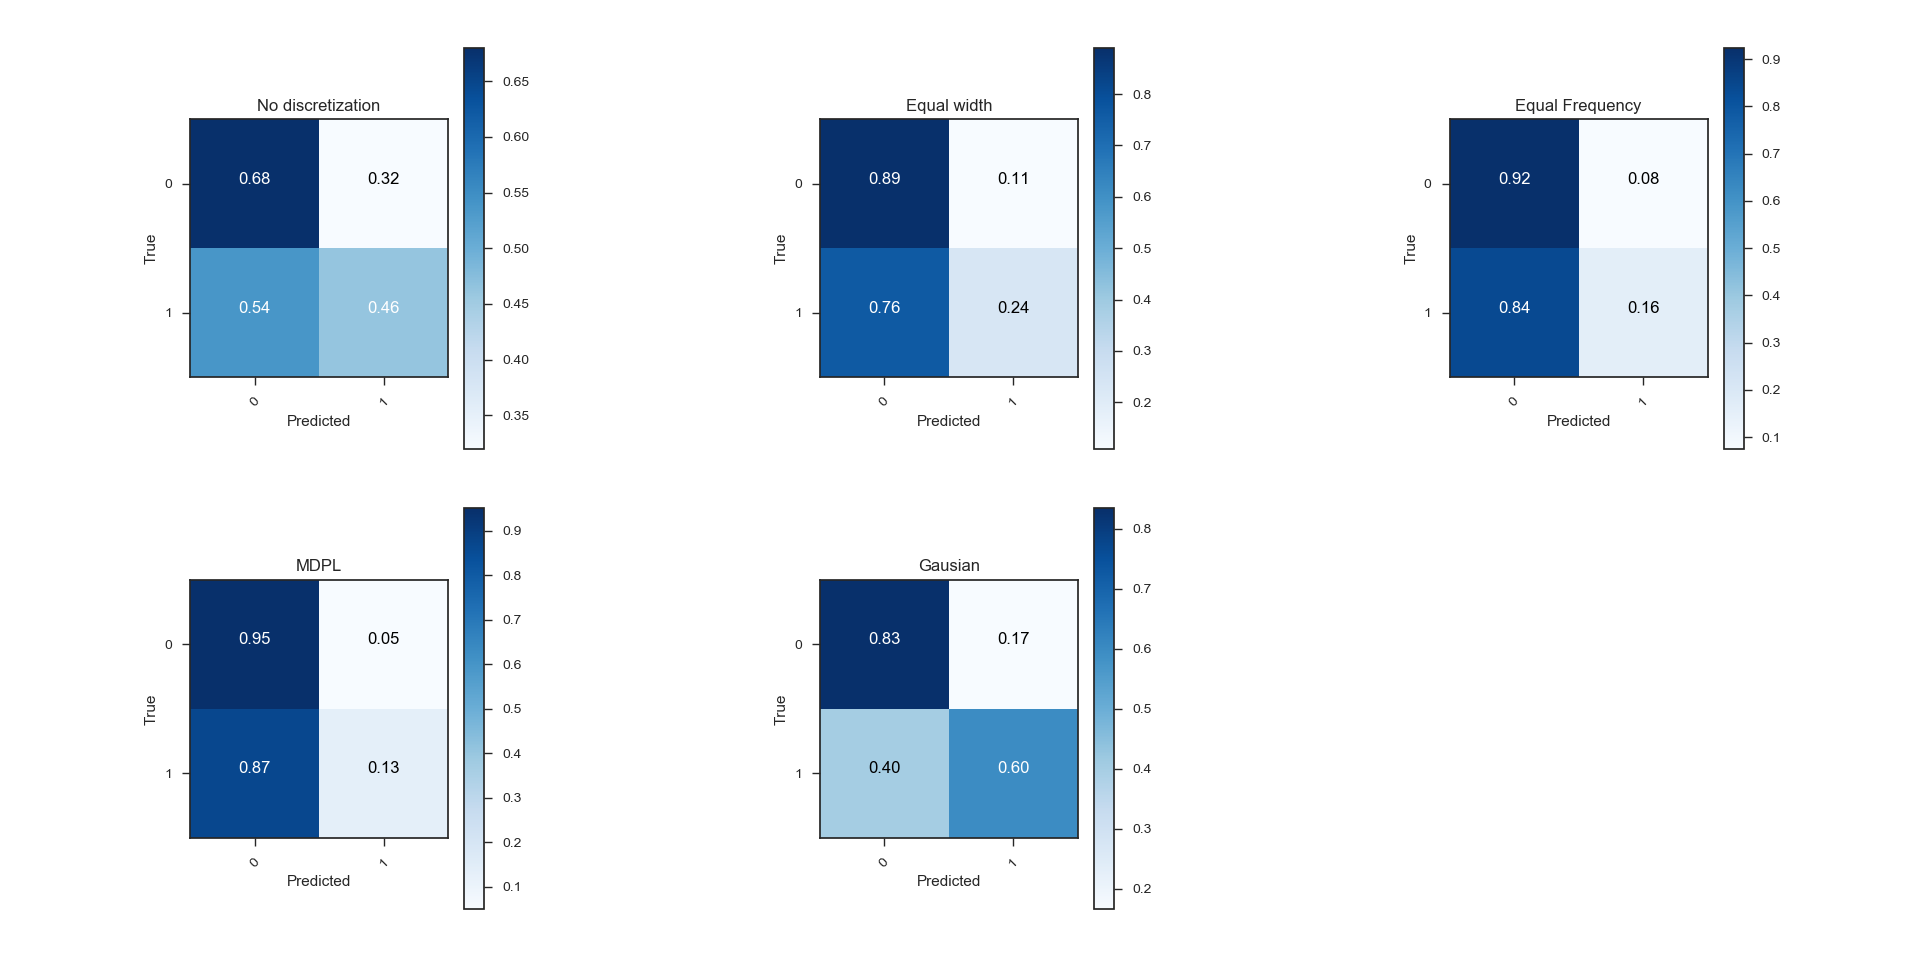
\includegraphics[width=1\textwidth]{diabetesCM.png}
\caption{Confusion Matrix dla instancji Diabetes}
\end{figure}





\section{Wnioski}
W ramach zadania zaimplementowany został naiwny klasyfikator bayesa. Dobór metody liczenia prawdopodobieństwa oraz dyskretyzacji, a także parametrów dyskretyzacji zależy od badanej instancji. W przypadku zbioru Wine oraz Diabetes użycie \emph{GausianNB} dawało o wiele lepsze wyniki niż użycie \emph{MultinomialNB} niezależnie od wybranych współczynników metod dyskretyzacji.\\
Natomiast w przypadku instancji \emph{Glass} znacząco lepsze rezultaty daje zastosowanie \emph{MultinomialNB}, a ponadto odpowiednia metoda dyskretyzacji jeszcze bardziej wpływa na polepszenie jakości klasyfikatora. W wypadku instancji \emph{Glass} metoda dyskretyzacji \emph{MDLP} wpłynęła na poprawienie wyników o prawie 20\% względem  braku dyskretyzacji oraz o około 8\% względem drugiej najlepszej w tym przypadku metody \emph{equal frequency}.\\
W przypadku klasyfikacji danych w realnym świecie ważne jest, zdarzają się przypadki, w których większy nacisk kładziony jest na poprawną klasyfikację do danej klasy, kosztem błędnej klasyfikacji pozostałych próbek. W przypadku diagnozowania chorób lepiej, aby osobę chorą skierować na dodatkowe badania mimo tego, że nie cierpi na żadną chorobę, niż przeoczyć chorobę u osoby, u której w rzeczywistości występuje.\\
W przypadku sposobu oceny klasyfikatora \emph{k-fold crossvalidation} jest dobrą metodą, szczególnie w wersji stratyfikowanej, gdzie ilość części nie odgrywa szczególnego znaczenia. W przypadku wersji niestratyfikowanej ważne jest, aby przemieszać dane, ponieważ sztywno określona kolejność zwykle skutkuje tym, że dane o podobnych cechach znajdują się w jednej z części co w rezultacie daje nam wyniki, które nie pokrywają się z realną jakością klasyfikatora. Ilość części, na które dzielimy zbiór powinna być nie mniejsza niż ilość klas w zbiorze. Najlepszą decyzją jest jednak posłużenie się kroswalidacją stratyfikowaną.

\end{document}





























